% ARGUS IEEE conference manuscript
% Overleaf: create a blank project, upload main.tex and references.bib, then compile with pdfLaTeX.
% Replace the author block below with the final author names, affiliation, and contact details.
\documentclass[conference]{IEEEtran}

\usepackage{amsmath,amssymb,amsfonts}
\usepackage{booktabs}
\usepackage{multirow}
\usepackage{graphicx}
\usepackage{array}
\usepackage{cite}
\usepackage{url}
\usepackage{xcolor}
\usepackage{tikz}
\usetikzlibrary{arrows.meta,positioning,fit,calc,shapes.geometric}
\usepackage{pgfplots}
\usepgfplotslibrary{groupplots}
\pgfplotsset{compat=1.18}

\definecolor{argusblue}{RGB}{32,119,189}
\definecolor{arguscyan}{RGB}{30,190,190}
\definecolor{argusorange}{RGB}{230,126,34}
\definecolor{argusred}{RGB}{196,53,53}
\definecolor{argusgreen}{RGB}{35,150,90}
\definecolor{argusgray}{RGB}{78,86,98}

\newcommand{\vect}[1]{\boldsymbol{#1}}
\newcommand{\E}{\mathbb{E}}
\newcommand{\R}{\mathbb{R}}
\newcommand{\eps}{\varepsilon}
\newcommand{\Hn}{\bar{H}}
\newcommand{\argus}{\textsc{Argus}}
\newcommand{\code}[1]{\texttt{#1}}
\newcolumntype{L}[1]{>{\raggedright\arraybackslash}p{#1}}

\title{ARGUS: Cost-Aware Closed-Loop Bayesian Experiment Design\\
for Adaptive Acoustic Defect Localization}

\author{%
\IEEEauthorblockN{Ripan}
\IEEEauthorblockA{Independent Researcher\\India}
}

\begin{document}
\maketitle

\begin{abstract}
Most data-driven nondestructive-evaluation systems passively classify a fixed measurement. This paper presents ARGUS (Adaptive Recursive Guided Uncertainty Sensing), a working research prototype that instead closes the loop between sensing and inference: it maintains a spatial posterior over a hidden defect, predicts which candidate source--receiver experiment will best separate the leading hypotheses, executes that experiment, recursively updates the posterior, and stops when confidence or an experiment budget is reached. The prototype combines an interpretable direct-plus-scattered acoustic digital twin, matched-filter delay likelihoods, a $20\times20$ Bayesian belief grid, a counterfactual response-signature planner, physical-motion and repetition costs, a domain-randomized neural forward surrogate, four acquisition backends, and a browser scientific-instrument interface. In a paired benchmark of 30 medium-difficulty simulated panels and a ten-measurement budget, ARGUS reduced normalized entropy from 1.000 to 0.419, compared with 0.498 for random probing and 0.621 for a uniform grid. Mean localization error was 12.33 mm versus 13.38 mm and 13.26 mm, respectively; however, bootstrap intervals for the error advantages crossed zero, so the defensible result is improved uncertainty concentration rather than a proven localization advantage. A synthetic forward surrogate achieved mean held-out feature $R^2=0.409$. An adapter for the public LMSD 2021 CFRP dataset produced 294 measured-response channels; scenario-held-out mean $R^2=0.001$ exposed the remaining sim-to-real gap. These results establish an end-to-end, reproducible active-sensing platform while clearly delimiting what remains to be validated on blind physical defects.
\end{abstract}

\begin{IEEEkeywords}
active sensing, Bayesian experimental design, structural health monitoring, nondestructive evaluation, information gain, guided waves, uncertainty quantification, digital twin, adaptive measurement
\end{IEEEkeywords}

\section{Introduction}
Nondestructive evaluation (NDE) is usually presented as a mapping from a measurement to a decision: acquire a waveform, compute features, and classify or localize damage. That formulation leaves the measurement geometry fixed. Yet the source position, receiver position, waveform, frequency band, amplitude, and duration determine which aspects of an internal structure are observable. When measurements have different costs, choosing the next experiment can be as important as interpreting the previous one.

ARGUS addresses the sequential question
\begin{equation}
 e_{t+1}^{\star}=\arg\max_{e\in\mathcal{E}_{t}}
 \left[\mathcal{I}_t(e)-\mathcal{C}_t(e)\right],
 \label{eq:intro-objective}
\end{equation}
where $e$ is a physically executable experiment and $\mathcal{E}_{t}$ is a state-dependent candidate set. After observing response $y_{t+1}$, ARGUS performs a recursive Bayesian update, regenerates candidates from the new posterior, and repeats. This is related to Bayesian experimental design and active data selection \cite{chaloner1995,mackay1992}, but instantiated as a live, spatial, source--receiver interrogation loop.

The prototype targets an opaque rectangular panel with one dominant hidden anomaly (cavity, loose region, delamination, or dense inclusion). Its central distinction from a one-shot classifier is summarized in Table~\ref{tab:comparison}. It is designed to run without hardware through a seeded physics-inspired simulator, while the same session engine accepts a microphone, validated WAV upload, or serial-connected probe.

\begin{table}[t]
\caption{Passive Detection Versus ARGUS Active Interrogation}
\label{tab:comparison}
\centering
\small
\begin{tabular}{@{}L{0.20\columnwidth}L{0.27\columnwidth}L{0.42\columnwidth}@{}}
\toprule
Property & Passive pipeline & ARGUS prototype \\
\midrule
Measurement & Fixed plan & Chosen from current belief \\
State & Label or point & Normalized spatial posterior \\
Uncertainty & Often implicit & Entropy, covariance, local mass \\
History & Optional aggregation & Recursive Bayesian fusion \\
Output & Detect or locate & Map, next action, reason, stop state \\
Efficiency & Scan or fixed network & Information--cost tradeoff \\
\bottomrule
\end{tabular}
\end{table}

The contributions of this implementation are:
\begin{enumerate}
    \item a complete observe--infer--plan--act loop joining acoustic response simulation or acquisition to recursive spatial belief updating;
    \item a cost-aware Adaptive Physical Experiment Planner that compares counterfactual delay, attenuation, and phase signatures of the top-$K$ posterior hypotheses;
    \item a numerically safeguarded likelihood engine based on baseline subtraction, FFT correlation, robust scaling, signal-to-noise-dependent tempering, and Bayesian fusion;
    \item a reproducible evaluation against random and uniform-grid policies, including paired uncertainty trajectories and confidence intervals;
    \item an operational bridge from simulation to physical research through interchangeable acquisition devices, ESP32 firmware, calibration, planar camera guidance, persistent sessions, and an adapter for a licensed experimental CFRP dataset.
\end{enumerate}

The novelty claim is deliberately narrow. Guided-wave NDE, Bayesian sensor placement, active learning, and matched filtering all predate this work \cite{rose2014,flynn2010,turin1960}. The research contribution is their particular real-time composition around movable source--receiver experiments, competing posterior hypotheses, explicit action costs, recursive stopping, and inspectable rationales. Legal patentability is not established by this manuscript and requires a professional claim-specific prior-art search.

\section{Related Work and Design Position}
\subsection{Guided-Wave and Vibration-Based Inspection}
Elastic waves can interrogate plate-like structures over areas larger than a probe footprint, while damage modifies propagation through scattering, attenuation, mode conversion, and local resonance \cite{rose2014}. Practical guided-wave interpretation is complicated by dispersion, anisotropy, boundaries, coupling variability, and environmental drift. Open Guided Waves provides controlled CFRP measurements for comparative algorithm research \cite{moll2019}, illustrating both the value and the complexity of measured wavefields.

ARGUS does not claim that its compact simulator is a high-fidelity Lamb-wave or finite-element model. It uses path length, propagation delay, attenuation, signed defect reflection, frequency-sensitive gain, and damped ringing to create an interpretable inverse problem that can exercise the complete adaptive loop. The real-device path is intentionally decoupled from this simulator.

\subsection{Bayesian Design and Active Measurement}
Bayesian experimental design selects an experiment according to expected utility under current uncertainty \cite{chaloner1995}; information-based active selection chooses data expected to be informative about hypotheses or predictions \cite{mackay1992}. In structural health monitoring, Flynn and Todd formulated optimal actuator/sensor placement using Bayes risk and demonstrated active guided-wave examples \cite{flynn2010}. Much of that literature optimizes a fixed network or configuration. ARGUS instead replans a single next, executable experiment after every observation and incorporates movement, excitation, and redundancy costs.

Exact expected information gain would marginalize over all possible future observations for every candidate. That calculation is expensive and only as reliable as the generative model. ARGUS therefore uses a bounded counterfactual-disagreement proxy. Throughout this paper, ``expected information gain'' means this implemented proxy, not an exact mutual-information calculation or a guarantee of global optimality.

\subsection{Open Experimental Evidence}
The LMSD 2021 dataset contains measured frequency-response functions (FRFs) from a $600\times600\times4$ mm cross-ply CFRP plate, a $12\times12$ coordinate grid, seven accelerometer/hammer nodes, a healthy baseline, and six added-mass scenarios \cite{dwek2024dataset}. It supplies real multistatic responses and known mass locations, but not cavities, delaminations, or adaptively selected trials. ARGUS uses it to test data ingestion and feature transfer, not to imply physical validation of every supported defect type.

\section{Problem Formulation}
Let the panel occupy normalized coordinates $\Omega=[0,1]^2$. Physical distance is evaluated after the transformation
\begin{equation}
 \vect{p}_{\mathrm{m}}=\mathrm{diag}(W,H)\vect{p},
 \label{eq:physical-map}
\end{equation}
where the default width and height are $W=0.60$ m and $H=0.40$ m. The latent defect state is
\begin{equation}
 z=(x,y,r_x,r_y,q,T),
\end{equation}
containing center, elliptical radii, severity $q\in[0,1]$, and type $T$. The current prototype explicitly infers only location $(x,y)$ on an $G\times G$ grid; size, severity, and type are nuisance variables captured by simulator randomization and likelihood robustness.

An experiment is
\begin{equation}
 e=(\vect{s},\vect{r},f_0,f_1,a,d,w),
\end{equation}
where $\vect{s}$ and $\vect{r}$ are normalized source and receiver coordinates, $f_0,f_1$ are band endpoints, $a$ is normalized amplitude, $d$ is duration, and $w\in\{\text{impulse,sine,chirp}\}$. Given observation history $\mathcal{D}_t=\{(e_i,y_i)\}_{i=1}^{t}$, the belief grid is
\begin{equation}
 P_t(j)=P(z_{xy}=j\mid\mathcal{D}_t),\qquad
 \sum_{j=1}^{G^2}P_t(j)=1.
\end{equation}
The initial belief is uniform. Each observation supplies a likelihood $L_{t+1}(j)$ and
\begin{equation}
 P_{t+1}(j)=\frac{P_t(j)\max[L_{t+1}(j),\eps]}
 {\sum_kP_t(k)\max[L_{t+1}(k),\eps]},\quad \eps=10^{-12}.
 \label{eq:bayes}
\end{equation}
The normalized uncertainty is
\begin{equation}
 \Hn(P)=-\frac{\sum_jP(j)\log_2(P(j)+\eps)}{\log_2(G^2)}\in[0,1].
 \label{eq:entropy}
\end{equation}

\section{System Architecture}
Figure~\ref{fig:architecture} shows the implemented data flow. Ground truth exists only inside simulation sessions and remains server-side until an explicit reveal action. Both simulated and physical signals pass through the same analysis, persistence, and user-interface contracts.

\begin{figure*}[t]
\centering
\resizebox{0.94\textwidth}{!}{%
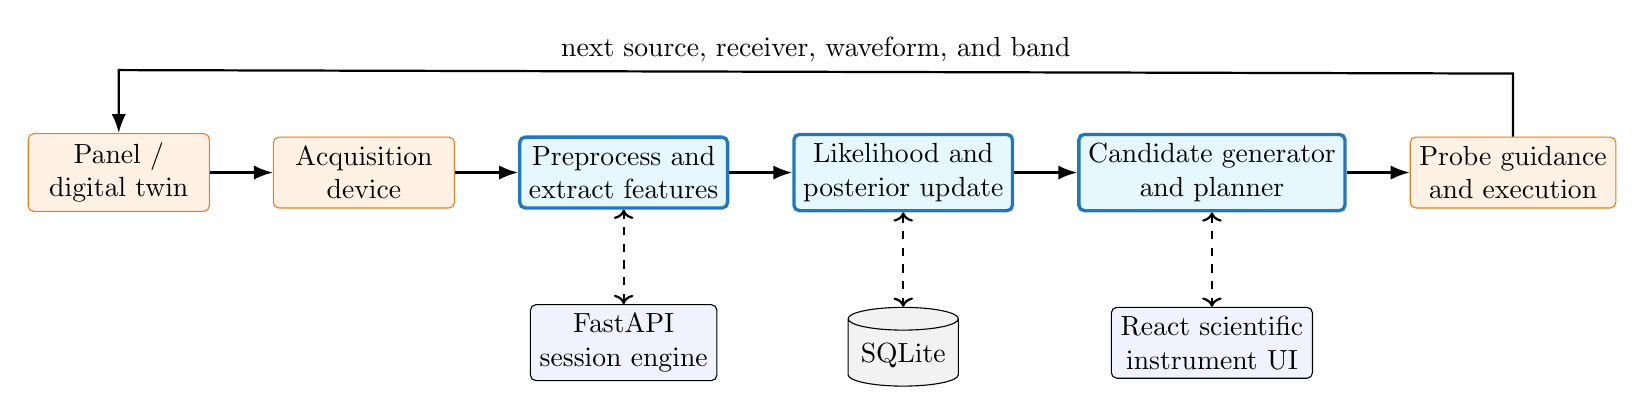
\begin{tikzpicture}[
node distance=7mm and 8mm,
block/.style={draw,rounded corners=2pt,align=center,minimum height=9mm,minimum width=23mm,fill=blue!5},
core/.style={block,fill=cyan!10,draw=argusblue,very thick},
io/.style={block,fill=orange!10,draw=argusorange},
store/.style={cylinder,shape border rotate=90,draw,aspect=0.22,minimum height=10mm,minimum width=14mm,fill=gray!10},
arr/.style={-{Latex[length=2.4mm]},thick}
]
\node[io] (world) {Panel /\\digital twin};
\node[io,right=of world] (device) {Acquisition\\device};
\node[core,right=of device] (signal) {Preprocess and\\extract features};
\node[core,right=of signal] (belief) {Likelihood and\\posterior update};
\node[core,right=of belief] (planner) {Candidate generator\\and planner};
\node[io,right=of planner] (guidance) {Probe guidance\\and execution};
\node[store,below=12mm of belief] (db) {SQLite};
\node[block,below=12mm of signal] (api) {FastAPI\\session engine};
\node[block,below=12mm of planner] (ui) {React scientific\\instrument UI};
\draw[arr] (world)--(device);
\draw[arr] (device)--(signal);
\draw[arr] (signal)--(belief);
\draw[arr] (belief)--(planner);
\draw[arr] (planner)--(guidance);
\coordinate (loopright) at ($(guidance.north)+(0,8mm)$);
\coordinate (loopleft) at ($(world.north)+(0,8mm)$);
\draw[arr] (guidance.north)--(loopright)--node[above,align=center]{next source, receiver, waveform, and band}(loopleft)--(world.north);
\draw[<->,dashed,thick] (api)--(signal);
\draw[<->,dashed,thick] (belief)--(db);
\draw[<->,dashed,thick] (planner)--(ui);
\end{tikzpicture}}
\caption{ARGUS closed-loop architecture. The planner changes the next physical experiment; it does not merely classify a fixed waveform.}
\label{fig:architecture}
\end{figure*}

The Python backend contains domain models, simulation, signal analysis, belief inference, planning, evaluation, device adapters, session orchestration, and SQLite persistence. A FastAPI layer exposes session, recommendation, experiment, upload, posterior, history, reveal, device, and benchmark endpoints. The TypeScript/React frontend visualizes the posterior heatmap, recommended geometry, signal, spectrum, power spectral density, spectrogram, belief history, benchmark curves, and camera overlay. A single launcher starts both processes locally.

\section{Physics-Inspired Forward Model}
\subsection{Excitation}
For $N=\lfloor d f_s\rceil$ samples at default sample rate $f_s=16$ kHz, the excitation occupies the first
\begin{equation}
 N_b=\left\lfloor f_s\min(10\,\mathrm{ms},0.22d)\right\rceil
\end{equation}
samples. A Tukey window with shape parameter 0.45 suppresses burst discontinuities \cite{harris1978}. A sine uses $\sin(2\pi f_0t)$; a chirp sweeps linearly from $f_0$ to $f_1$; and the impulse option uses a Ricker-like pulse
\begin{align}
 u(t)&=a[1-2\phi(t)^2]\exp[-\phi(t)^2],\\
 \phi(t)&=\frac{\pi(t-0.28d_b)}{\max(f_c^{-1},0.22\,\mathrm{ms})}.
\end{align}

\subsection{Direct and Scattered Responses}
Let $d_{sr}$ denote physical source--receiver distance and let $d_{sz},d_{zr}$ denote the two legs through the defect. The response is
\begin{equation}
 y(t)=A_0u(t-\tau_0)+A_zu(t-\tau_z)+r_z(t)+n(t)+b(t),
 \label{eq:forward}
\end{equation}
with fractional delays obtained by linear interpolation. For wave velocity $c$, attenuation $\alpha$, and system delay $t_0$,
\begin{align}
 \tau_0 &= t_0+d_{sr}/c,& A_0&=\frac{e^{-\alpha d_{sr}}}{1+4d_{sr}},\\
 \tau_z &= t_0+(d_{sz}+d_{zr})/c.&
\end{align}
The defect resonance and scattered gain are
\begin{align}
 f_z &= f_{\mathrm{mat}}(1.05-0.32q),\\
 R_f &=0.72+0.72\exp\!\left[-\frac{1}{2}
 \left(\frac{f_c-f_z}{1250}\right)^2\right],\\
 A_z &=0.43\rho_Tq\frac{\sqrt{r_xr_y}}{0.085}
 \frac{e^{-\alpha(d_{sz}+d_{zr})}}{1+5(d_{sz}+d_{zr})}R_f,
 \label{eq:scatter}
\end{align}
where $\rho_T=1.00,0.72,0.86,-0.64$ for cavity, loose region, delamination, and dense inclusion, respectively. The negative dense-inclusion coefficient creates a phase inversion. Starting at $\tau_z$,
\begin{equation}
 r_z(t)=0.11 A_z a\sin[2\pi f_r(t-\tau_z)]e^{-\beta(t-\tau_z)},
\end{equation}
where $f_r=f_z$ except for dense inclusions, for which $f_r=1.12f_z$. Noise $n(t)$ is Gaussian; $b(t)$ is a cumulative low-frequency random drift. The default material values are $c=180$ m/s, $\alpha=1.65$ m$^{-1}$, $f_{\mathrm{mat}}=3100$ Hz, $\beta=95$ s$^{-1}$, $t_0=0.8$ ms, and noise standard deviation 0.007.

This model is intentionally identifiable and fast enough for interactive candidate evaluation. It omits dispersion branches, anisotropic stiffness, boundary-mode conversion, transducer electromechanics, and spatially varying coupling. Consequently, simulation accuracy must not be confused with field accuracy.

\section{Signal Interpretation and Recursive Belief}
\subsection{Preprocessing and Features}
The pipeline rejects nonfinite or shorter-than-eight-sample signals, removes the mean, and optionally applies a fourth-order zero-phase Butterworth bandpass from 250 Hz to $\min(7000,0.96f_s/2)$ Hz. Peak normalization is optional and disabled for feature extraction so amplitude remains informative. A Hann-windowed real FFT produces a unit-sum spectral energy distribution. Welch PSD, a short-time spectrogram, and a Hilbert envelope support inspection \cite{welch1967,oppenheim1999}.

Table~\ref{tab:features} lists the 15 learned forward-response targets. The runtime inspector additionally returns a robust noise estimate. Low-, mid-, and high-band fractions span 250--1500, 1500--3500, and 3500--7000 Hz (clipped by Nyquist). Spectral entropy is normalized by the log of the number of FFT bins. Decay time is the first post-envelope-peak sample below $1/e$ of the peak. The noise scale is $1.4826$ times the median absolute deviation (MAD) in the first 10\% of the record.

\begin{table}[t]
\caption{ARGUS Response Features}
\label{tab:features}
\centering
\small
\begin{tabular}{L{0.32\columnwidth}L{0.58\columnwidth}}
\toprule
Group & Features \\
\midrule
Amplitude & RMS, peak, crest factor \\
Temporal & zero-crossing rate, envelope-peak time, $1/e$ decay time \\
Spectral shape & centroid, bandwidth, 85\% rolloff, dominant frequency, normalized entropy \\
Spectral allocation & low-, mid-, and high-band energy fractions \\
Quality & RMS-to-robust-noise SNR in dB \\
\bottomrule
\end{tabular}
\end{table}

\subsection{Matched-Filter Spatial Likelihood}
The inference engine subtracts the predicted healthy direct response, giving residual $v=y-\hat y_0$. It correlates $v$ with the excitation using an FFT implementation, retains nonnegative lags, takes absolute magnitude, and applies a seven-sample maximum filter. Correlation is the classical matched-filter operation for a known waveform in noise \cite{turin1960}.

For every grid-cell center $j$, the model predicts the bistatic delay
\begin{equation}
 \hat\tau_j=t_0+\frac{d(\vect{s},\vect{z}_j)+d(\vect{z}_j,\vect{r})}{c}.
 \label{eq:bistatic}
\end{equation}
The correlation value at the nearest nonnegative lag is assigned to that cell, smoothed spatially by a Gaussian with $\sigma=0.55$ cells, and robustly scaled between its 8th and 98th percentiles to $\tilde C_j\in[0,1]$. The likelihood is
\begin{align}
 L(j)&\propto \exp(T_{\mathrm{eff}}\tilde C_j),\\
 T_{\mathrm{eff}}&=4.8\,\mathrm{clip}\!\left(
 \frac{\mathrm{SNR}-0.75}{1.8},0.30,1\right),
 \label{eq:likelihood}
\end{align}
where SNR is residual RMS divided by residual MAD scale. Scaling $L$ to have mean one makes the Bayesian update numerically convenient without altering Eq.~\eqref{eq:bayes}.

\subsection{Estimation, Confidence, and Termination}
ARGUS reports both the maximum-a-posteriori (MAP) grid center and posterior mean. The $2\times2$ covariance is the posterior-weighted covariance of cell coordinates and yields a confidence ellipse. Let $m_{\mathrm{local}}$ be posterior mass in a square neighborhood of radius $\max(1,\lfloor G/16\rfloor)$ around the MAP cell. The displayed confidence is the bounded heuristic
\begin{equation}
 Q=\mathrm{clip}\{0.55m_{\mathrm{local}}+0.45[1-\Hn(P)],0,1\}.
 \label{eq:confidence}
\end{equation}
The default controller stops when $Q\ge0.72$, $\Hn(P)\le0.38$, or 12 experiments have been executed. A benchmark may impose a different budget; the reported study used ten.

\section{Adaptive Physical Experiment Planner}
\subsection{Candidate Construction}
The generator mixes eight perimeter locations with the eight highest-posterior cells as candidate sources. Receivers are the four perimeter corners plus the center. It cycles through bands 1.2--3.0, 2.2--4.4, and 3.4--6.2 kHz, with chirp, impulse, and chirp waveforms, amplitudes 0.42, 0.48, or 0.54, and 0.12 s duration. Near-coincident source--receiver pairs are redirected. Duplicate parameter tuples are removed until the default pool contains 48 candidates.

\subsection{Counterfactual Hypothesis Disagreement}
Let $\mathcal{K}$ contain the top $K=24$ grid hypotheses, with represented posterior mass $M=\sum_{i\in\mathcal{K}}P(i)$ and normalized weights $w_i=P(i)/M$. For candidate $e$, the fast forward signature is
\begin{equation}
 \vect{g}_i(e)=\left[\tau_i,\log(A_i+10^{-8}),\sin\varphi_i,\cos\varphi_i\right],
 \quad \varphi_i=2\pi f_c\tau_i,
 \end{equation}
where $A_i=0.65e^{-\alpha d_i}/(1+5d_i)$. Delay and log-gain dimensions are divided by 0.18 ms and 0.55, respectively, while sine/cosine encode circular phase without wrap discontinuities. With scaled signature $\tilde{\vect g}$, pairwise distinguishability and disagreement are
\begin{align}
 D_{ij}(e)&=1-\exp\left[-\tfrac12\|\tilde{\vect g}_i(e)-\tilde{\vect g}_j(e)\|_2^2\right],\\
 D(e)&=\sum_{i,j\in\mathcal{K}}w_iw_jD_{ij}(e).
 \label{eq:disagreement}
\end{align}
The bounded information-gain proxy is
\begin{equation}
 I(e)=H(P)M D(e),
 \label{eq:eig}
\end{equation}
in bits. It grows with current uncertainty, posterior mass represented by the leading hypotheses, and predicted separability. It is not the expected value of Eq.~\eqref{eq:entropy} under a calibrated observation distribution.

Candidate coverage is
\begin{equation}
 U(e)=\sum_{i\in\mathcal{K}}w_i\exp[-2.2\min(d_{si},d_{ir})].
\end{equation}
The implemented physical cost is
\begin{equation}
 C(e)=0.52a^2\frac{d}{0.12}+0.48\frac{\|\vect{s}-\vect{s}_{t}\|_2}{\sqrt2},
 \label{eq:cost}
\end{equation}
with zero motion term for the first experiment. Redundancy is the closest match to any previous experiment:
\begin{equation}
 R(e)=\max_{h<t}\exp[-6\|\vect{s}-\vect{s}_h\|_2]
 \exp[-2|f_c-f_{c,h}|/3000].
 \label{eq:repeat}
\end{equation}
The final score is
\begin{equation}
 S(e)=I(e)+0.35D(e)+0.22U(e)-0.16C(e)-0.22R(e).
 \label{eq:planner}
\end{equation}
The highest-scoring candidate is selected. The interface exposes all terms for the top five candidates, preventing the planner from becoming an opaque recommendation engine.

\begin{figure}[t]
\centering
\begin{minipage}{0.98\columnwidth}
\hrule
\vspace{1mm}
\noindent\textbf{Algorithm 1: ARGUS closed-loop localization}\par
\small
\begin{tabular}{@{}r p{0.88\columnwidth}@{}}
1: & \textbf{Input:} panel model, stopping thresholds, budget $B$.\\
2: & Set $P_0(j)\gets1/G^2$ and $\mathcal{D}\gets\emptyset$.\\
3: & \textbf{for} $t=0,\ldots,B-1$ \textbf{do}\\
4: & \quad Form sources from perimeter and leading cells.\\
5: & \quad Generate and deduplicate candidate experiments.\\
6: & \quad Retain top-$K$ posterior hypotheses.\\
7: & \quad \textbf{for each} candidate $e$ \textbf{do}\\
8: & \qquad Predict $\{\vect g_i(e)\}_{i=1}^{K}$.\\
9: & \qquad Compute $I(e),D(e),U(e),C(e),R(e)$.\\
10: & \qquad $S(e)\gets I+.35D+.22U-.16C-.22R$.\\
11: & \quad \textbf{end for}\\
12: & \quad Set $e_{t+1}\gets\arg\max_eS(e)$ and execute it.\\
13: & \quad Acquire $y_{t+1}$ and construct $L_{t+1}$.\\
14: & \quad $P_{t+1}\gets\mathrm{normalize}(P_t\odot L_{t+1})$.\\
15: & \quad Persist signal, features, scores, and posterior.\\
16: & \quad \textbf{break if} confidence or entropy threshold holds.\\
17: & \textbf{end for}\\
18: & \textbf{Return:} MAP, mean, covariance, confidence, history.\\
\end{tabular}
\vspace{1mm}
\hrule
\end{minipage}
\label{alg:argus}
\end{figure}

\subsection{Programmatic Explanation}
The selected recommendation receives a deterministic rationale. High disagreement produces a competing-regions explanation; broad entropy produces a coverage explanation; otherwise the system describes local ambiguity resolution. If repetition is below 0.25 after prior measurements, the explanation notes that the geometry and frequency avoid recent experiments. No language model is required, and every statement traces to planner state.

\section{Learned Forward Surrogate and Data}
\subsection{Domain-Randomized Synthetic Set}
The optional learned component approximates expected response features, not the final posterior. Each row contains 24 inputs describing defect state, panel/material nuisance variables, and experiment parameters, and 15 outputs from Table~\ref{tab:features}. Three thousand examples were generated with locations in $[0.08,0.92]^2$, radii 0.04--0.14, severity 0.35--0.96, all four defect types, panel sizes 0.45--0.85 by 0.30--0.60 m, velocity 145--245 m/s, attenuation 1.0--2.4 m$^{-1}$, resonance 2.5--4.2 kHz, damping 70--135 s$^{-1}$, noise 0.003--0.014, and randomized probes, bands, amplitudes, and waveforms.

The PyTorch \cite{paszke2019} network is
\begin{equation}
 24\rightarrow96\rightarrow96\rightarrow15,
\end{equation}
with SiLU activations and LayerNorm after the first hidden layer. Inputs and targets are standardized on training statistics. Training uses Smooth L1 loss, AdamW at learning rate $1.8\times10^{-3}$ and weight decay $10^{-4}$, batch size 128, a seeded 70/15/15 split, and early stopping. The physics predictor remains the default planner model because it is interpretable and the surrogate has uneven feature accuracy.

\subsection{Measured LMSD Adapter}
The downloader queries the official Zenodo record, downloads declared NPZ files, and verifies each published MD5 checksum. The adapter converts each complex 0--1600 Hz FRF to a 0.12 s impulse response, normalizes known node coordinates, encodes the added mass as a dense inclusion, and extracts the same feature contract. Six scenarios times seven sources times seven receivers yield 294 channels. To prevent leakage, splitting is by entire damage scenario: 196 training, 49 validation, and 49 test channels. These channels are correlated views of six physical damage configurations, not 294 independent defects.

\section{Physical and Software Realization}
\subsection{Acquisition Abstraction}
All devices implement connect, disconnect, acquire, and status operations. \code{SimulationDevice} executes Eq.~\eqref{eq:forward}; \code{MicrophoneDevice} records through the local audio stack; \code{UploadedSignalDevice} accepts WAV files; and \code{SerialProbeDevice} performs a line-framed transaction with an ESP32. Missing audio or serial hardware is reported without disabling simulation.

Uploads are limited to 10 MB, checked for allowed media types, decoded in memory, downmixed to mono, resampled by polyphase filtering, checked for finite values, and padded or truncated to the configured duration. The API never accepts arbitrary filesystem paths. Simulation ground truth is omitted from ordinary session payloads until reveal.

\subsection{Calibration and Coordinates}
The calibration routine executes three chirps across distinct geometries and estimates noise standard deviation, effective propagation velocity, baseline RMS, and resonance. Values are persisted in the panel's calibration profile. Normalized coordinates keep the planner independent of physical dimensions, while the UI presents millimeters using Eq.~\eqref{eq:physical-map}.

A camera-guidance mode asks the operator to click the four panel corners in top-left, top-right, bottom-right, bottom-left order. Eight homography parameters are solved from the four point correspondences \cite{hartley2004}. The browser overlays the recommended source, receiver, and posterior estimate on the planar image. This is operator guidance, not metrology; corner error and perspective uncertainty are not propagated into the current posterior.

\subsection{ESP32 Probe}
The reference firmware uses GPIO25 for an exciter-driver control, GPIO34 for a conditioned analog sensor, GPIO2 for status, and 115200 baud serial. It accepts \code{PING} and an \code{EXPERIMENT} command containing frequency, amplitude, duration, waveform, and sample rate, then returns \code{BEGIN}, framed \code{DATA}, and \code{END}. An exciter must be driven through a MOSFET/transistor or amplifier; it must not be powered directly from a GPIO. A piezo input requires current limiting, clamping, biasing, and conditioning so the ADC never sees negative voltage or an overvoltage transient.

\subsection{Persistence and Reproducibility}
SQLite stores session configuration, calibration, compressed floating-point responses, extracted features, candidate scores, posterior history, and random-generator state. NumPy/SciPy provide vectorized numerics and signal processing \cite{harris2020,virtanen2020}. Fixed seeds cover defect generation, observation noise, dataset splitting, training, and benchmark policy comparison. The API schema and saved JSON/CSV results allow an independent run to inspect every reported metric.

\section{Evaluation Protocol}
The evaluation addresses four questions:
\begin{itemize}
    \item \textbf{RQ1:} Does active planning concentrate spatial belief faster than random or uniform probing?
    \item \textbf{RQ2:} Does lower uncertainty translate into lower localization error under the same budget?
    \item \textbf{RQ3:} Can a small learned surrogate reproduce domain-randomized signal features?
    \item \textbf{RQ4:} Do those learned features transfer across held-out physical damage scenarios?
\end{itemize}

For RQ1--RQ2, 30 medium-preset defects were generated with seeds 100--129. Each of three policies operated on the identical hidden defect for a maximum of ten measurements. \emph{Random} sampled continuous source and receiver positions and a frequency band. \emph{Uniform grid} followed a fixed geometry sequence. \emph{ARGUS} used Eq.~\eqref{eq:planner}. Policies were compared using mean and median localization error, normalized final entropy, entropy reduction, entropy area under the measurement curve (AUC), physical cost, experiment count, and success within 10, 15, 20, and 30 mm. Paired bootstrap 95\% intervals were computed over the shared cases. No assertion required error to improve monotonically.

For RQ3, the 3000-example synthetic model used seed 23 and independent random splitting. For RQ4, the LMSD model used the same architecture and seed but held out complete scenarios. Smooth L1 values across these two data regimes are not directly comparable because their target statistics and split difficulty differ.

\section{Results}
\subsection{Planner Benchmark}
Table~\ref{tab:benchmark} reports the saved benchmark, not hand-entered target values. ARGUS achieved the lowest mean error, final entropy, entropy AUC, and mean experiment count. At 15 mm it localized 73.3\% of cases, versus 56.7\% for random and 60.0\% for the grid. At 20 mm all methods reached 93.3\%; therefore the strongest separation occurs at the tighter 15 mm criterion.

\begin{table*}[t]
\caption{Paired Simulation Benchmark: 30 Medium-Preset Defects, Ten-Experiment Budget}
\label{tab:benchmark}
\centering
\small
\begin{tabular}{lrrrrrrrrr}
\toprule
Policy & Mean error & Median error & Mean exp. & Final $\Hn$ & Entropy red. & Entropy AUC & Cost & $\le15$ mm & $\le20$ mm \\
 & (mm) & (mm) & & & & & & (\%) & (\%) \\
\midrule
Random & 13.38 & 14.44 & 10.00 & 0.498 & 0.502 & 0.748 & 2.665 & 56.7 & 93.3 \\
Uniform grid & 13.26 & 13.84 & 10.00 & 0.621 & 0.379 & 0.818 & \textbf{2.481} & 60.0 & 93.3 \\
ARGUS & \textbf{12.33} & \textbf{13.28} & \textbf{9.83} & \textbf{0.419} & \textbf{0.581} & \textbf{0.740} & 2.588 & \textbf{73.3} & 93.3 \\
\bottomrule
\end{tabular}
\end{table*}

Relative to random probing, ARGUS lowered final entropy by 15.9\%, lowered mean error by 7.8\%, and used 2.9\% less modeled cost. Relative to the grid, it lowered final entropy by 32.5\% and mean error by 7.0\%, but used 4.3\% more modeled cost. The result illustrates Eq.~\eqref{eq:intro-objective}: information efficiency and physical cost are related but distinct objectives.

Figure~\ref{fig:trajectories} shows mean trajectories. ARGUS does not dominate localization error at every intermediate step; its mean error is especially high after the second measurement and briefly rises again after the sixth. This is permissible in a noisy recursive estimator and reinforces why entropy and error must both be reported.

\begin{figure*}[t]
\centering
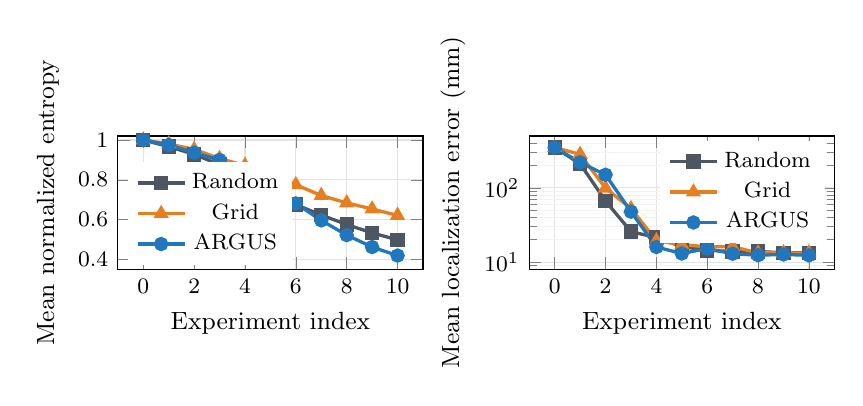
\begin{tikzpicture}
\begin{groupplot}[
group style={group size=2 by 1,horizontal sep=1.35cm},
width=0.45\textwidth,height=0.27\textwidth,
xlabel={Experiment index},grid=both,minor grid style={gray!10},major grid style={gray!22},
tick label style={font=\footnotesize},label style={font=\small},legend style={font=\footnotesize,draw=none},
xtick={0,2,4,6,8,10}
]
\nextgroupplot[ylabel={Mean normalized entropy},ymin=0.35,ymax=1.02,legend pos=south west]
\addplot[very thick,argusgray,mark=square*] coordinates {(0,1.000)(1,.967)(2,.928)(3,.876)(4,.810)(5,.747)(6,.675)(7,.623)(8,.575)(9,.533)(10,.498)};
\addlegendentry{Random}
\addplot[very thick,argusorange,mark=triangle*] coordinates {(0,1.000)(1,.980)(2,.953)(3,.907)(4,.872)(5,.832)(6,.775)(7,.721)(8,.684)(9,.653)(10,.621)};
\addlegendentry{Grid}
\addplot[very thick,argusblue,mark=*] coordinates {(0,1.000)(1,.975)(2,.936)(3,.900)(4,.837)(5,.755)(6,.681)(7,.596)(8,.522)(9,.462)(10,.419)};
\addlegendentry{ARGUS}
\nextgroupplot[ylabel={Mean localization error (mm)},ymode=log,ymin=8,ymax=500,legend pos=north east]
\addplot[very thick,argusgray,mark=square*] coordinates {(0,350.386)(1,211.182)(2,66.588)(3,25.742)(4,21.415)(5,16.194)(6,14.408)(7,13.875)(8,13.870)(9,13.379)(10,13.379)};
\addlegendentry{Random}
\addplot[very thick,argusorange,mark=triangle*] coordinates {(0,350.386)(1,283.198)(2,99.231)(3,52.709)(4,19.419)(5,17.126)(6,16.121)(7,16.081)(8,13.322)(9,13.322)(10,13.259)};
\addlegendentry{Grid}
\addplot[very thick,argusblue,mark=*] coordinates {(0,350.386)(1,220.503)(2,150.202)(3,47.800)(4,15.970)(5,13.053)(6,15.215)(7,12.966)(8,12.390)(9,12.685)(10,12.331)};
\addlegendentry{ARGUS}
\end{groupplot}
\end{tikzpicture}
\caption{Mean uncertainty (left) and localization-error (right, logarithmic axis) trajectories over the same 30 hidden defects. Lower is better.}
\label{fig:trajectories}
\end{figure*}

Paired results in Table~\ref{tab:paired} qualify the aggregate means. ARGUS reduced final entropy in 28/30 cases versus random and 30/30 versus grid, with both confidence intervals above zero. In contrast, both mean-error intervals include zero and strict error win rate is 30\%. Thus RQ1 is supported in this simulator, while RQ2 remains suggestive rather than statistically established. Tied MAP cells and a few large improvements explain why mean error can improve despite a low strict-win fraction.

\begin{table}[t]
\caption{Paired ARGUS Advantages (95\% Bootstrap CI)}
\label{tab:paired}
\centering
\small
\resizebox{\columnwidth}{!}{%
\begin{tabular}{lrrr}
\toprule
Comparison & Mean error advantage (mm) & Mean entropy advantage & Win rate (error / entropy) \\
\midrule
vs. random & 1.048 $[-0.667,2.812]$ & 0.079 $[0.063,0.095]$ & 0.30 / 0.93 \\
vs. grid & 0.928 $[-1.021,2.757]$ & 0.202 $[0.180,0.224]$ & 0.30 / 1.00 \\
\bottomrule
\end{tabular}}
\end{table}

\subsection{Forward-Surrogate Results}
The synthetic surrogate stopped at epoch 27. Table~\ref{tab:ml} shows that amplitude, decay, and SNR-related features are learnable under domain randomization, while dominant frequency and envelope timing are poorly captured. Mean feature $R^2=0.409$ is useful as an engineering diagnostic but not sufficient justification to replace the physics signature in safety-relevant planning.

The measured LMSD scenario-held-out result is much weaker: mean $R^2=0.001$ and standardized MAE 0.449. High-band energy alone achieved $R^2=0.875$; many other features were negative out of sample. The adapter therefore demonstrates an honest data path and exposes domain shift rather than validating physical generalization. In particular, test Smooth L1 0.190 should not be interpreted as better than the synthetic 0.225 because the standardized targets and held-out units differ.

\begin{table}[t]
\caption{Learned Forward-Response Evaluation}
\label{tab:ml}
\centering
\small
\resizebox{\columnwidth}{!}{%
\begin{tabular}{lrrrll}
\toprule
Data & Samples & Test Smooth L1 & Std. MAE & Mean $R^2$ & Split \\
\midrule
Synthetic & 3000 & 0.2245 & 0.5014 & 0.4092 & seeded 70/15/15 \\
LMSD measured & 294 & 0.1902 & 0.4485 & 0.0010 & held-out scenario \\
\bottomrule
\end{tabular}}
\vspace{1mm}

\footnotesize Synthetic best $R^2$: SNR 0.910, RMS 0.861, peak 0.825, crest 0.758, decay 0.622. Synthetic weak examples: dominant frequency $-0.019$, envelope-peak time 0.016.
\end{table}

\subsection{Software Verification}
The executed verification suite contains 19 backend tests covering deterministic simulation, normalized posterior updates, entropy, candidate validity, planning, signal processing, feature extraction, API lifecycle, persistence, surrogate loading, and data contracts. The frontend passed lint and production build; package audit reported zero known vulnerabilities; Python dependency checking passed; and live HTTP checks reached the frontend and health endpoint. The only observed test warning is an upstream deprecation notice in the HTTP test client, not a runtime failure.

\section{Why the Design Is Novel and Useful}
The system-level research hypothesis is that hidden-state inference becomes more measurement-efficient when the AI controls the interrogation itself. Five aspects distinguish the implemented prototype:
\begin{enumerate}
    \item \textbf{Actionable uncertainty:} the posterior is not only visualized; it directly generates source positions and top competing hypotheses.
    \item \textbf{Counterfactual physical discrimination:} candidates are scored by how different the predicted responses would be if each leading spatial hypothesis were true.
    \item \textbf{Resource-aware recursion:} amplitude, duration, probe movement, and repetition enter the same decision as informativeness.
    \item \textbf{Inspectability:} the top five decomposed scores, deterministic rationale, signal diagnostics, and entire belief history are exposed.
    \item \textbf{Modality boundary:} device and session interfaces separate acquisition from inference, allowing the closed-loop pattern to extend to thermal, impedance, RF, optical, or tactile measurements without treating those modalities as already implemented.
\end{enumerate}

The potentially protectable technical nucleus, subject to legal review, is not ``AI for defect detection'' or ``information gain'' in isolation. It is the concrete sequence that (i) derives leading spatial hypotheses from a recursively updated physical belief, (ii) predicts candidate-specific multicomponent physical response signatures under those counterfactual hypotheses, (iii) jointly penalizes excitation, movement, and redundancy, (iv) executes the selected real experiment, and (v) repeats until an uncertainty-based stop condition while retaining an auditable explanation. Prior art may disclose some or all of these elements in adjacent combinations; only a professional search can determine novelty and non-obviousness for particular claims.

\section{Limitations and Threats to Validity}
\subsection{Model and Inference Limits}
The simulator is nondispersive and uses a single effective velocity. A real composite plate supports multiple dispersive, anisotropic modes and boundary reflections. The location-only grid assumes one dominant anomaly; it does not infer a no-defect state, defect count, shape, type, or severity. Baseline subtraction assumes the nominal digital twin is sufficiently calibrated. Multiplying successive likelihoods also assumes conditional independence given location, while shared model error can make confidence over-sharp.

Confidence in Eq.~\eqref{eq:confidence} is a heuristic mixture, not a calibrated posterior coverage probability. The planner's Eq.~\eqref{eq:eig} is a ranking proxy, and its constants were engineered rather than learned from physical utility. A future system should use posterior predictive calibration, model discrepancy variables, likelihood tempering learned on held-out specimens, and abstention when measured signals are out of distribution.

\subsection{Evaluation Limits}
Thirty synthetic cases provide a useful paired smoke test, not a population-scale validation. The mean-error confidence intervals cross zero; no claim of superior physical localization is warranted. The baselines are intentionally simple and do not include advanced tomography, Gaussian-process Bayesian optimization, reinforcement learning, or optimal fixed-array design. Hyperparameters were not evaluated in a nested holdout, and the benchmark shares the simulator assumptions used by inference.

The LMSD experiment has only six independent damage scenarios, several with multiple masses. Hammer/accelerometer FRFs at 0--1600 Hz differ from the prototype's 1.2--6.2 kHz chirp interrogation. Added masses are scattering surrogates, not cavities or delaminations. Scenario-held-out performance correctly reveals that correlated channel count cannot replace independent physical diversity.

\subsection{Operational Limits}
Microphone measurements are vulnerable to airborne sound and ambient noise. Probe remounting changes coupling. Camera homography assumes a planar stationary panel and accurate clicks. ESP32 analog acquisition needs safe conditioning and synchronized excitation. The prototype is not certified NDE equipment and must not be used as the sole basis for safety-critical maintenance decisions.

\section{Physical Validation and Data-Collection Plan}
A credible next study should use at least three nominally identical panels, eight repeatably mounted perimeter transducers, an instrumented exciter, five repeats per condition, and healthy measurements before and after each damage block. Reversible bonded masses, damping patches, or paired magnets are appropriate for commissioning. True cavities or delaminations require manufactured specimens---for example flat-bottom holes or embedded release films---and independent truth from ultrasound, radiography, or destructive sectioning where justified.

For the current acquisition contract, collect all 56 ordered non-self source--receiver pairs, three frequency bands, and five repeats. One physical state yields $56\times3\times5=840$ waveforms. Twenty known locations plus healthy references yield approximately 17,000 signals. Preserve raw waveforms and record specimen, material, thickness, defect geometry and truth method, source and receiver coordinates, excitation, repeat, temperature, humidity, coupling force, remount identifier, calibration, timestamp, and code version.

Split development data by complete defect location, stronger validation by complete specimen, and the final test by a blind panel whose truth remains hidden until predictions and stopping decisions are frozen. Offline planner evaluation additionally needs a complete counterfactual bank: every admissible experiment must be recorded for every hidden state so all policies query the same physical response table. Report error versus measurement budget, entropy calibration, success radii, abstention, remount robustness, and temperature shift.

\section{Reproducibility}
The repository provides commands for the complete workflow:
\begin{verbatim}
python run_argus.py
python scripts/demo_simulation.py
python scripts/evaluate_model.py
python scripts/generate_dataset.py
python scripts/train_model.py
python scripts/download_lmsd_dataset.py
python scripts/prepare_lmsd_dataset.py
pytest
\end{verbatim}
The externally downloaded data are intentionally excluded from version control; DOI, license, source filenames, and checksums are preserved. Trained metadata records seeds, split units, sample counts, feature names, per-feature MAE, and $R^2$. Benchmark JSON preserves per-case trajectories as well as summary values.

\section{Conclusion}
ARGUS demonstrates that an NDE prototype can be organized around the next experiment rather than only the next prediction. The implemented loop chooses a source, receiver, band, amplitude, duration, and waveform from a recursive belief; acquires or simulates a response; updates a spatial posterior; explains the decision; and stops under explicit uncertainty and budget rules. In the current matched-model simulation, the planner concentrates belief more consistently than random or uniform probing, while localization-error superiority remains unproven. The measured CFRP adapter further shows that sim-to-real transfer is the central research risk. The most valuable next milestone is therefore a preregistered, specimen-held-out, blind physical campaign with a full counterfactual measurement bank and calibrated uncertainty. That experiment would test the core proposition: whether adaptive physical interrogation can obtain a reliable defect map with fewer, safer, and more informative measurements.

\section*{Acknowledgment}
The authors acknowledge the LMSD group at KU Leuven for releasing the LMSD 2021 plate-damage dataset under CC BY 4.0. Dataset use in ARGUS retains the published DOI and provenance.

\appendices
\section{Default Configuration}
\refstepcounter{table}
\label{tab:defaults}
\begin{center}
\footnotesize
\textsc{Table \Roman{table}}\\
\textsc{Important Reproducible Defaults}
\vspace{1mm}

\centering
\renewcommand{\arraystretch}{0.97}
\begin{tabular}{@{}L{0.20\columnwidth}L{0.43\columnwidth}L{0.27\columnwidth}@{}}
\toprule
Subsystem & Parameter & Value \\
\midrule
Panel & width $\times$ height & $0.60\times0.40$ m \\
Material & velocity & 180 m/s \\
Material & attenuation & 1.65 m$^{-1}$ \\
Material & resonance & 3100 Hz \\
Material & damping & 95 s$^{-1}$ \\
Material & noise standard deviation & 0.007 \\
Material & system delay & 0.8 ms \\
Signal & sample rate & 16 kHz \\
Signal & record duration & 0.12 s \\
Belief & grid; base temperature & $20\times20$; 4.8 \\
Stop & confidence; normalized entropy & 0.72; 0.38 \\
Stop & maximum experiments & 12 \\
Planner & candidate count; top hypotheses & 48; 24 \\
Planner & $I,D,C,R$ weights & 1, .35, .16, .22 \\
Planner & coverage weight & 0.22 \\
Easy & radii; severity; noise multiplier & .10--.15; .78--.95; .55 \\
Medium & radii; severity; noise multiplier & .065--.11; .58--.82; 1.0 \\
Hard & radii; severity; noise multiplier & .04--.075; .38--.64; 1.55 \\
Reproducibility & default seed & 7 \\
\bottomrule
\end{tabular}
\end{center}

\section{Interpretation Guide for Demonstrations}
An entropy decrease means probability mass has concentrated, not necessarily that the mode is correct. Confidence combines concentration and local mass but is not a certified probability of correctness. Ground truth should remain hidden until the controller stops. The reveal should report physical error using panel dimensions, not normalized distance. If entropy falls while revealed error remains high, the correct diagnosis is model mismatch or an overconfident likelihood, not a successful run.

The strongest concise description for a judge is: ``ARGUS is an AI-guided scientific instrument that decides which physical measurement to take next. It predicts where competing defect hypotheses would respond differently, trades that information against movement and excitation cost, performs the experiment, and recursively sharpens a visible probability map.'' The strongest defensible evidence statement is: ``In 30 paired simulated cases, ARGUS ended with lower entropy than random in 28 cases and lower than the grid in all 30; physical generalization is the next validation milestone.''

\IEEEtriggeratref{6}
\bibliographystyle{IEEEtran}
\bibliography{references}

\end{document}
